%%
%% This is file `sample-sigplan.tex',
%% generated with the docstrip utility.
%%
%% The original source files were:
%%
%% samples.dtx  (with options: `sigplan')
%% 
%% IMPORTANT NOTICE:
%% 
%% For the copyright see the source file.
%% 
%% Any modified versions of this file must be renamed
%% with new filenames distinct from sample-sigplan.tex.
%% 
%% For distribution of the original source see the terms
%% for copying and modification in the file samples.dtx.
%% 
%% This generated file may be distributed as long as the
%% original source files, as listed above, are part of the
%% same distribution. (The sources need not necessarily be
%% in the same archive or directory.)
%%
%% The first command in your LaTeX source must be the \documentclass command.
\documentclass[sigplan,screen,nonacm]{acmart}
\usepackage{listings}

\makeatletter
\def\subsubsection{\@startsection{subsubsection}{3}%
  \z@{.5\linespacing\@plus.7\linespacing}{.1\linespacing}%
  {\normalfont\itshape}}
\makeatother

%Code listing style named "mystyle"
\lstdefinestyle{mystyle}{
  commentstyle=\color{codegreen},
  keywordstyle=\color{magenta},
  stringstyle=\color{codepurple},
  basicstyle=\ttfamily\footnotesize,
  breakatwhitespace=false,         
  breaklines=true,                 
  captionpos=b,                    
  keepspaces=true,                 
  numbers=left,                    
  numbersep=5pt,                  
  showspaces=false,                
  showstringspaces=false,
  showtabs=false,                  
  tabsize=2,
  frame = single
}
%"mystyle" code listing set
\lstset{style=mystyle}

%%
%% \BibTeX command to typeset BibTeX logo in the docs
\AtBeginDocument{%
  \providecommand\BibTeX{{%
    \normalfont B\kern-0.5em{\scshape i\kern-0.25em b}\kern-0.8em\TeX}}}

%%
%% end of the preamble, start of the body of the document source.
\begin{document}

%%
%% The "title" command has an optional parameter,
%% allowing the author to define a "short title" to be used in page headers.
\title{Saving 25\% Memory Usage via Radix Trees in FoundationDB, a Highly-Performant Distributed Key-Value Store}

%%
%% The abstract is a short summary of the work to be presented in the
%% article.
\begin{abstract}
With the cost of main memory constantly decreasing, larger and larger databases can now be stored and accessed primarily in memory. This memory-centric paradigm brings new challenges to the way data should be stored and indexed in main memory in order to be processed efficiently. Traditional in-memory data structures like balanced binary search trees are not optimized for modern hardware, due to poor cache utilization. Moreover, they are not very space-efficient for datasets that involve a large amount of prefix-overlap in keys. Hash tables, another popular in-memory key-value storage data structure, are fast for update and lookup operations, but only support single-key queries without more powerful functionality such as range scans. 

This paper presents the development of a new in-memory storage engine based on the radix tree data structure for FoundationDB (FDB), an open-source highly scalable distributed key-value store in heavy use at Wavefront by VMWare and other leading companies like Apple, Inc.  Our trie-based index structure uses compact and adaptive data representations for tree nodes to reduce the memory footprint while supporting efficient lookups and updates. The experimental evaluation shows that our optimized radix-tree storage engine consumes 25\% less memory than the original binary search tree design for highly concurrent workloads and is able to maintain performance at the same time. 

Our radix tree engine has been contributed upstream within the FoundationDB open source project and will be added as a second memory storage engine inside FDB. Any applications that use FDB as their underlying distributed database can switch to this new storage engine with little to zero modification.
 
\end{abstract}

%%
%% Keywords. The author(s) should pick words that accurately describe
%% the work being presented. Separate the keywords with commas.
% \keywords{Main-memory key-value stores, index structures, radix tree, Wavefront}

%%
%% This command processes the author and affiliation and title
%% information and builds the first part of the formatted document.
\maketitle

\section{Introduction}
\label{sec:intro}
After decades of development in modern hardware, commodity servers with terabytes of RAM are widely available at affordable prices, making main-memory database systems possible. For main-memory database systems, having fast and space-efficient index structures is crucial in order to achieve high overall performance, and thus has prompted a considerable amount of research in the area. While Red-black trees \cite{bayer1972symmetric} or T-trees \cite{lehman1985study} were first proposed as index data structures and once very popular, some modern in-memory systems (e.g., Silo \cite{tu2013speedy} or HyPer \cite{kemper2011hyper}) choose trie structures (e.g., Masstree \cite{mao2012cache} or ART \cite{leis2013adaptive}). The reason behind this preference is that traditional binary search trees like Red-black trees suffer from poor cache behaviors \cite{rao1998cache} and usually require additional rebalancing operations. Well-engineered tries, on the other hand, are aware of cache misses and tend to be more space-efficient using prefix compression. Moreover, unlike hash tables that scatter the keys randomly, tries are order-preserving and therefore support range scans and related operations (e.g., prefix lookup or top-k).

The goal of this paper is to describe the design and implementation of a new FDB main-memory storage engine based on the radix tree index structure. 

Radix Tree is a space-optimized trie, which achieves its low memory consumption via {\itshape vertical compression}. By vertical compression, each node in radix tree that is an only child is merged with its parent to help reduce the tree height. However, this requires a trade-off between tree height and space efficiency by setting a globally valid span parameter. For a given span {\itshape s}, keys are split into partial keys of {\itshape s} bits each and inner nodes usually use an array of $2^{s}$ to store child pointers. The problem of a larger span value is wasted space consumption as most of the pointers in the nodes will be empty and the actual fanout is typically much smaller than the optimal number (i.e., $2^{s}$). ART \cite{leis2013adaptive} overcome this shortcoming using adaptive inner nodes (also known as {\itshape horizontal compression}) where the inner node type is dynamically decided by the number of children. 

We show in this paper how to implement a variant of adaptive inner nodes specifically tuned for the Wavefront workloads. We follow the high-level strategy of creating different inner node types but simplify the conversion logic and merge some types into one using more compact node representations. Furthermore, other additional optimizations, including in-line data that leverages the {\itshape union} type, bit fields  \cite{oualline1997practical} and replacing std::map with std::vector, allow Wavefront radix tree to further decrease space usage by avoiding unnecessary memory/heap allocation. 

This work makes the following contributions:
\begin{itemize}
\item We implement the radix tree memory storage engine, a general-purpose store that supports various operations (including point queries, range queries, and incremental updates), but is particularly optimized for space efficiency. 
\item We experimentally compare the radix tree memory storage engine with the default binary search tree design in FDB for concurrent Wavefront workloads. The results show that our implementation has reduced 25\% memory consumption while maintaining the overall performance. 
\item We’ve integrated our new memory storage engine into the open-source FDB project.
\end{itemize}

\section{Background}
In this section, we give a general description of the FDB storage architecture, to see how our radix tree index structure fits into the big picture. Then introduce Wavefront and its workload properties, explaining the motivations to develop a trie-based memory storage engine. 

\subsection{FDB Storage Architecture}
FoundationDB \cite{fdb} is a distributed database designed to handle large volumes of structured data across clusters of commodity servers. It organizes data as an \textbf{ordered} key-value store and employs ACID transactions for all operations. In FDB storage landscape, there is a {\itshape distributed transaction log system} (TLog) and we have a {\itshape storage server} role, as illustrated in Figure \ref{fig:FDB-storage-architecture}. The outermost layer is storage server which receives mutations in version order from TLogs and constantly applies them to {\itshape storage engine}. The storage engine lives inside the storage sever, and each storage server contains exactly one instance of it. Its main purpose is to persist key-value pairs into disk. For a memory storage engine specifically, data goes directly into {\itshape key-value container} in main memory, while all operations are logged to disk to guarantee durability. One of the intriguing properties of storage engine is that it’s used by a single process on one thread, and therefore simplifies the development as there is no need to worry about concurrency issues. The key-value container sits at the lowest level in the FDB storage architecture, having no knowledge about transactions and existing only an index structure that helps store and retrieve data efficiently. For the FDB current implementation, it’s a balanced binary search tree, where keys are stored in lexicographical order. 
\begin{figure}[t]
  \centering
  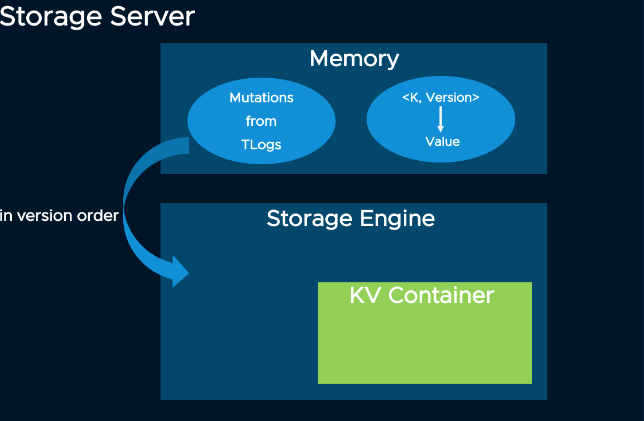
\includegraphics[width=\linewidth, height=6cm]{pic/FDB-storage-architecture.png}
  \setlength{\abovecaptionskip}{-10pt} 
  \setlength{\belowcaptionskip}{-7pt} 
  \caption{FDB storage server key components, where the key-value container is essentially the index structure.}
  \label{fig:FDB-storage-architecture}
\end{figure}

\subsection{Wavefront}
Wavefront \cite{wavefront} is a cloud-hosted monitoring platform that can ingest telemetry measurements such as {\itshape time series points} at a scale of millions per second. It uses FDB as primary means of storing data. Time series points in Wavefront have a payload consisting of a timestamp, a measurement value, a label of a customer name, a metric name, a host name, and an optional set of point tags. Figure \ref{fig:point-key} demonstrates an example of how Wavefront constructs a {\itshape point key}. One point is one row write, corresponding to one key-value pair inside FDB memory storage engine. However, the biggest problem of the default binary search tree memory storage engine is that there is zero prefix compression, meaning identical point labels (highlighted as a white box in Figure \ref{fig:point-key}) are stored multiple times. Given the high velocity of ingested telemetry data in Wavefront, this leads to a huge waste in memory usage. 
\begin{figure}[h]
  \centering
  
\includegraphics[width=\linewidth]{pic/point key.png}
  \setlength{\abovecaptionskip}{-10pt} 
  \setlength{\belowcaptionskip}{-7pt} 
  \caption{Example of a point key in Wavefront}
  \label{fig:point-key}
\end{figure}

\section{Implementation of Wavefront radix tree}
This section presents implementation details of our radix tree key-value container. We start with a deep dive into node structures, focusing on their functionalities and space consumption. Next, list key data structural enhancements we make in order to improve space efficiency.

\subsection{Node Structures}
In general, radix trees have two types of nodes. The first are inner nodes, which map partial keys to the next-level child. In a traditional implementation, inner nodes usually keep a fixed array of child pointers where the array size is controlled by the global span parameter s. This parameter is crucial for the performance of radix trees because it determines the tree height as well as the memory overhead for inner nodes. In our design, we choose the s = 8, corresponding to partial keys of 1 byte to avoid unnecessary bit shifting and masking operations. However, this choice could lead to a relatively high fanout rate thus excessive memory usage \cite{boehm2011efficient} , we tackle this problem by using adaptive inner nodes (details in section \ref{sec:inner-nodes}). The second type of node is leaf nodes, which store the values of each entry. In contrast to binary search trees, radix trees have several interesting properties (1) Nodes in radix trees do not contain complete keys; instead, they represent partial keys, and only the full path from the root to a leaf node describes the complete key corresponding to a value. (2) No rebalancing operations are ever needed. 

In our radix tree index structure design, there are three types of nodes:common nodes, inner nodes and leaf nodes. 

\subsubsection{Common Nodes}
In order to maintain a clean and well-structured code base, we create an extra node type that stores data shared by \textbf{both} inner and leaf nodes. Common nodes have {\itshape variable length partial keys} used for vertical compression. As mentioned in section \ref{sec:intro}, vertical compression is mainly realized by collapsing levels in the tree when an inner node has only one child. For example, in Figure \ref{fig:vertical-compression}, the inner node representing the partial key “C” was merged down. In such cases, the partial keys corresponding to the missing nodes are stored as our variable length keys inside common nodes. Other than partial keys, common nodes also keep some meta information, including a boolean that indicates whether this node is a leaf or not, an integer to keep track of the common prefix length with its ancestors and a parent pointer. The latter two are not mandatory but will help simplify and expedite the process of key reconstruction. 
\begin{figure}[t]
  \centering
  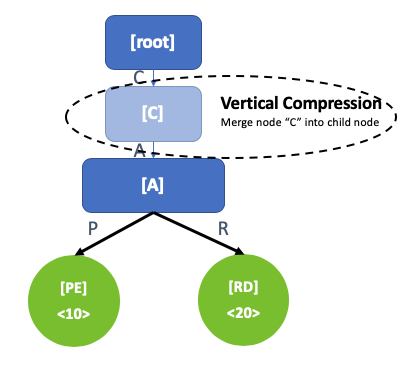
\includegraphics[width=\linewidth, height=6.5cm]{pic/vertical compression.png}
  \setlength{\belowcaptionskip}{-10pt} 
  \caption{Illustration of vertical compression for keys "cape" and "card". Inner node "C" has only one child, thus merging it downwards and update the partial keys}
  \label{fig:vertical-compression}
\end{figure}

\subsubsection{Inner Nodes}
\label{sec:inner-nodes}
Inspired by the concept of adaptive nodes, we use two data structures with different capacities to represent our inner node as shown in Figure \ref{fig:inner-nodes}. The idea is to choose node sizes dynamically and individually with respect to the actual fanout of the subtree underneath each node. 

\textbf {Inner Node3}: The smaller node type can store up to 3 partial keys using a fixed size array and child pointers are correspondingly stored at a separate array of the same size. Partial keys are sorted to support order-preserving operations like range scans. 

\textbf {Inner Node (Dynamic)}: The bigger node type can store between 4 and 256 entries using a dynamic array. Each entry is a combination of one partial key with its child pointer and the same as Node3 type, entries in the array are sorted based on partial keys. When inner nodes are first created, they always start with the Node3 type, as the number of children exceeds 3, they will automatically switch to the second type.  

Additionally, when it comes to space overhead, Node3 can have children size from 1 to 3 with a fixed overhead of 32 bytes (pointer in 64 bits platform is usually 8 bytes), while the Node (Dynamic) can have children size from 4 to 256 with a varying overhead from 88 to 4120 bytes. 
\begin{figure}[t]
  \centering
  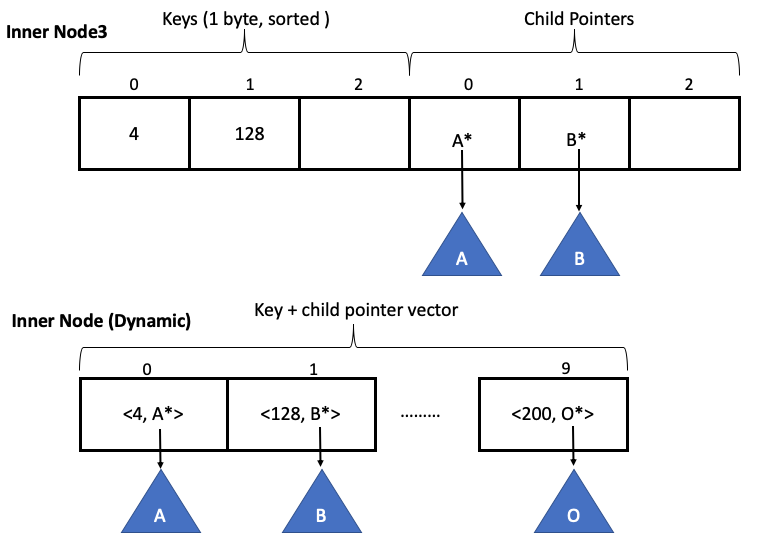
\includegraphics[width=\linewidth, height=6.5cm]{pic/inner nodes.png}
  \setlength{\belowcaptionskip}{-7pt} 
  \caption{Data representations for inner nodes. In both cases, partial keys 4, 128 are mapped to the next-level node A, B. But for Inner Node(Dynamic) type, it contains more entries.}
  \label{fig:inner-nodes}
\end{figure}

\subsubsection{Leaf Nodes}
Since FDB memory storage engine is a key-value store, our index structure must store the values associated with the corresponding keys. There are two different design choices: 
\begin{itemize}
    \item Option one : Get rid of the concept of value completely and store everything as variable length partial keys in common nodes. 
    \item Option two : Have a separate leaf node structure by adding value field inside the common node type. 
\end{itemize}
Figure \ref{fig:leaf-nodes} shows an example of two options. The second one is the more general method because it reduces the total number of nodes in radix trees by collapsing two into one. In our evaluation, we’ve tested with both implementations and found out the second one has smaller memory footprints. 
\begin{figure}[h]
  \centering
  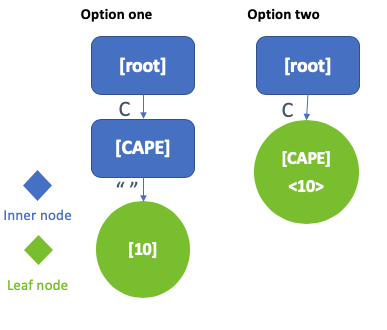
\includegraphics[width=\linewidth, height=5.5cm]{pic/leaf nodes.png}
  \setlength{\belowcaptionskip}{-10pt} 
  \caption{Example of two design options for leaf nodes. In both cases, we insert the same key-value pair.}
  \label{fig:leaf-nodes}
\end{figure}

\subsection{Other Optimizations}
\textbf {Bit Fields} : Different data types in C/C++ usually have different alignment requirements determined by the processor architecture. To maintain proper alignment in data structures, the complier normally inserts additional unnamed data members so that each member is properly aligned. For example, if you construct a data structure with one boolean and one double, system may end up allocating 16 bytes memory on 64-bit platform instead of 9 due to the padding. Structure padding could cause unnecessary overhead; However, the treatment of this problem is found by bit fields technique. The idea is to utilize the memory space efficiently by specifying the width of a variable in bits when we know the value will never exceed a limit. We use bit fields to better represent the meta information in common nodes and reduce the overhead from 24 bytes to 8 bytes.

\textbf {std::map VS. std::vector} : For inner Node (dynamic) type, we have two options in regards to storing partial keys and child pointers. std::map and std::vector are both dynamic data structures defined in STL C++, the former is a sorted key-value container ( usually implemented as red-black tree ) that requires additional memory usage for maintaining the structure while the latter is a sequence array, but in our case, we need to manually keep entries in order. We pick std::vector to save memory usage, and take advantage of binary search algorithm or SIMD instructions to speedup searching in the linearly-organized vector. 

\textbf {Inline Data} :  FDB uses a 12 bytes internal data structure called {\itshape StringRef} to represent keys and values. StringRef consists of two parts (1) An 8-byte pointer that points to a contiguous heap space allocated by the memory pool (2) An integer that defines the length. One observation from previous experiments is that around 80\% nodes in radix tree have the data length smaller than 12 bytes leading to the inline data optimization. We use a union type to store a StringRef member and a byte array of size 12. If the partial key size is smaller than 12 bytes, use byte array without allocating heap memory; If the partial key size is larger than 12 bytes, then switch to StringRef. 
% \begin{lstlisting}[language=C, caption=Example inline data]
% struct StringRef{
%     uint8_t *pointer;
%     int length;
% }
% union {
%     uint8_t inlineData[12];
%     StringRef data;
% }
% \end{lstlisting}

\section{Evaluation}
In this section, we evaluate our radix tree memory storage engine and compare it with the default balanced binary search tree implementation. We first describe the experimental setup before presenting our results, which focus on the following aspects: (1) memory consumption, (2) performance. 
 
\subsection{Testbed and Workloads}
Experiments were conducted on Wavefront internal testing cluster {\itshape mawenzi}. It consists of 6 database machines of i3.16xlarge instance type (64 vCPU, 488 GB RAM) and 42 FDB storage server processes. The maximum memory usage on each process is set to be 22GB. Furthermore, one of the useful properties of mawenzi is quad buffer configuration which means we could ingest data to 4 memory storage engines evenly using murmur3 hash to calculate the distribution. This setting gives us the ability to see how radix tree storage engine behaves against the default one, under the \textbf {exact same} workloads. In the following experiments, memory and memory 1 are set to be radix tree while memory 2 and memory 3 are set to be binary search tree. 

For our workloads, 
\begin{itemize}
    \item We use real-life Wavefront time series points generated by different customers. The average key length is 55 bytes and the value length is 8 bytes. Search, insert and delete operations are random. 
    \item We also test with a more generic dataset, the Wikipedia titles collection (295 MiB) \cite{wikidatasets}. This workload consists of inserting all the titles from the Wikipedia archive into two memory storage engines, check the used memory space after the insert and then search for all the entries again. Key is the title entry with average length 20 bytes and value is some randomly generated 8 bytes double. 
\end{itemize}

\subsection{Space Consumption}
Table \ref{tab:memory-usage} reports the memory consumption in MiB for two different storage engines. Memory consumption here is a metrics gather by the operating system, other than raw key-value size, it also includes node overhead, memory pool padding, data replication, etc. The table shows that for all datasets, radix tree outperforms the other implementation in terms of space efficiency. To be more specific, for Wavefront workloads, when the system stabilized, our radix tree store consumes 25\% less memory for \textbf {each} storage server process; for textual datasets, like the Wikipedia archive, our radix tree store still requires 20\% less space. 
\begin{table}[h]
  \caption{Memory consumption for storage engine types (in MiB)}
  \begin{tabular}{ccl}
    \toprule
    Storage engine type&Wavefront&Wikipedia\\
    \midrule
    Radix tree & 8,192 & 1,565\\
    Binary search tree & 11,264 & 1,974\\
    \bottomrule
  \end{tabular}
  \label{tab:memory-usage}
\end{table}

\begin{figure*}[t]
  \centering
  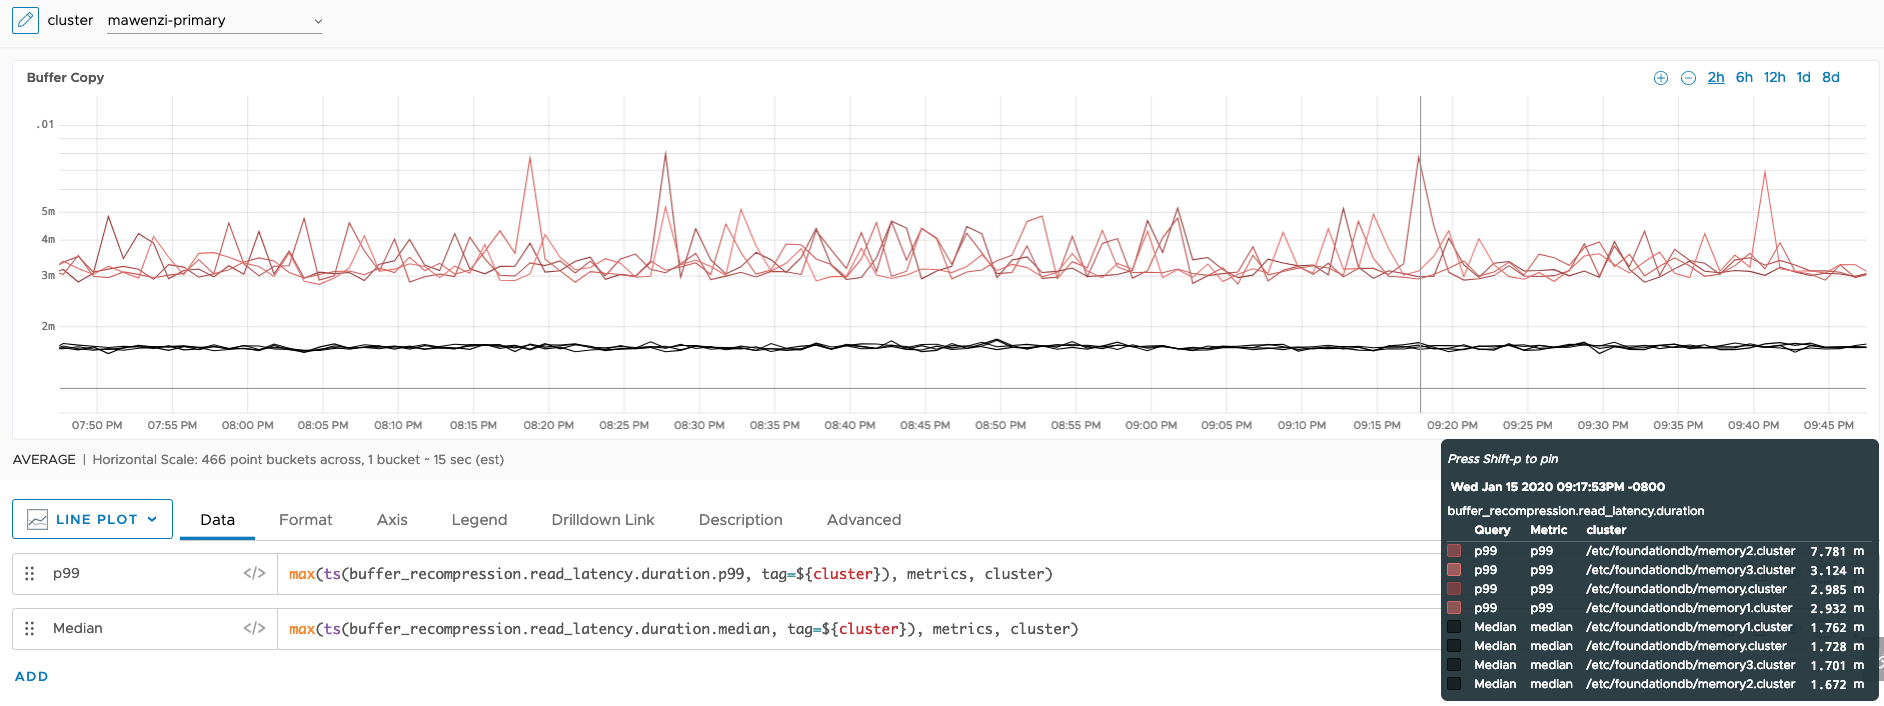
\includegraphics[width=\linewidth, height=6.5cm]{pic/read latency.png}
  \setlength{\belowcaptionskip}{-8pt} 
  \caption{Read latency values, including p99 and median, of different storage engines on mawenzi}
  \label{fig:read-latency}
\end{figure*}

\subsection{Performance}
Figure \ref{fig:read-latency} demonstrates the read latency for two different storage engines for Wavefront workloads. We measure the read latency for point queries and range queries on mawenzi cluster, then reporting it as a histogram. As shown in Figure \ref{fig:read-latency}, black lines represent the median value and the red lines represent the p99, two storage engine types have basically the same performance. Table \ref{tab:wiki-latency} records the insert and search latency for Wikipedia dataset. Overall, radix tree storage engine has comparable performance as the default one. 

\begin{table}[h]
  \caption{Lookup and insert operation latency}
  \begin{tabular}{ccl}
    \toprule
    Storage engine type&Lookup($\mu$s/key)&Insert($\mu$s/key)\\
    \midrule
    Radix tree & 0.61 & 1.81\\
    Binary search tree & 0.66 & 1.55\\
    \bottomrule
  \end{tabular}
  \label{tab:wiki-latency}
\end{table}

From these experiments, we conclude that besides featuring superior memory consumption in comparison with the default version, radix tree is still able to keep the search and update performance. 

\section{Conclusions and Future work}
In this paper, we show how to implement a fast and space-efficient FDB memory storage engine using the radix tree index structure. By taking advantage of a high fanout parameter and vertical compression, we’re able to reduce the tree height as well as the time complexity for search and update operations. Adaptive node representations, along with other optimizations like bit fields, inline data, limit the memory overhead and therefore lead to excellent space usage. Our experimental results show that the radix tree storage engine outperforms the default binary search tree in terms of space efficiency with at least 20\% saving. As for read-write performance, those two implementations have comparable results. 

In the future, we tend to add more aggressive methods to further decrease the node overhead. For example, use delta encoding algorithm for pointer representations. Also, we plan to implement optimizations for bulk deletions. Instead of erasing the node one by one, there is a quick way to delete subtree entirely.   

%%
%% The next two lines define the bibliography style to be used, and
%% the bibliography file.
\bibliographystyle{ACM-Reference-Format}
\bibliography{reference.bib}

\end{document}
\endinput
%%
%% End of file `radio-2020.tex'.
